\documentclass[11pt,a4paper]{article}

% ===== PACKAGES =====
\usepackage{fontspec}
\usepackage{amsmath,amssymb,amsfonts}
\usepackage{amsthm}
\usepackage{graphicx}
\usepackage{booktabs}
\usepackage{hyperref}
\usepackage{algorithm}
\usepackage{algpseudocode}
\usepackage{listings}
\usepackage[margin=1in]{geometry}

\usepackage{xcolor}
\usepackage{tikz}
\usetikzlibrary{arrows.meta, positioning, shapes.geometric}

\newtheorem{definition}{Definition}
\newtheorem{lemma}{Lemma}
\newtheorem{theorem}{Theorem}
\newtheorem{proposition}{Proposition}
\newtheorem{conjecture}{Conjecture}

% ===== METADATA =====
\title{Runtime Epistemic Control for Large Language Models\\A Semantic Validation Architecture for Bounded Deployment}

\author{
  Umut K\"{o}kg\"{o}z\\
  Akdeniz University -- Technology Transfer Office (TTO)\\
  KAIRA Research Initiative, Antalya, T\"{u}rkiye\\
  \texttt{umut@projectkaira.com}
  \and
  Cenk Tak{\i}m\\
  School of Foreign Languages\\
  Antalya Bilim University, T\"{u}rkiye\\
  \texttt{cenk.takim@antalya.edu.tr}
}

\date{April 2026}

\begin{document}

\maketitle

% ===== ABSTRACT =====
\begin{abstract}
Large Language Models (LLMs) are increasingly capable, but deployment risk is now shaped less by raw fluency than by control failure: overconfident false answers, unsupported operational instructions, unsafe tool invocation, and inability to signal uncertainty at runtime. This paper addresses that capability-versus-control gap in bounded operational environments. We present KAIRA (Knowledge Augmented Intelligent Rational Agent), a semantic validation architecture and constrained deployment runtime designed to govern high-capability LLMs in settings where unsupported outputs carry immediate operational cost.

KAIRA is not proposed as a replacement for foundation models, but as a deployment-time control architecture that constrains and audits their behavior in bounded operational environments. It operates as a runtime layer above an existing LLM. The architecture combines an Epistemic Control Layer (ECL), which estimates whether the system has enough grounded support to answer at all, with an Internal Deliberation Loop (IDL), which scores, critiques, and validates candidate outputs against a deterministic ontological graph and associated policy constraints. Low-support cases trigger refusal, clarification, deferred action, or human handoff rather than unconstrained generation. In this way, KAIRA treats deployment as a problem of semantic validation, uncertainty-aware action selection, and runtime governance.

We study the architecture in a service-domain setting, using hospitality automation as the primary deployment case. In a preliminary evaluation bounded to the ontology-covered domain, we observed an in-domain hallucination rate of 1.8\% under KAIRA compared to 12.4\% for the unconstrained baseline, with lower boundary-violation counts and higher response consistency. These figures are descriptive of the specific experimental setup and should not be interpreted as definitive performance guarantees. We also report a prototype deployment setting demonstrating constrained workflow execution and refusal behavior under live use. These results should be interpreted as preliminary evidence within the evaluated bounded domain; they do not imply open-domain reliability, universal truthfulness, or domain-general safety. The paper's central claim is narrower: high-capability LLMs can be made more governable in real deployments by placing epistemic gating, semantic validation, and bounded action policies at runtime.
\end{abstract}

\vspace{0.5em}
\noindent \textbf{Code \& Prototypes:} \url{https://github.com/umutkkgz/Kaira}

\textbf{Keywords:} AI Safety, Runtime Governance, Epistemic Control, Semantic Validation, Bounded Autonomy, Knowledge-Grounded Generation, Service Operations

% ===== I. INTRODUCTION =====
\section{Introduction}

The practical challenge in LLM deployment is no longer only capability. It is control. High-capability models can produce fluent and often useful responses, but the same generative mechanism also produces overconfident falsehoods, unsupported operational guidance, policy violations expressed in plausible language, and responses that conceal rather than expose uncertainty. These failures matter most in real deployments, where the cost of a wrong answer is borne by operators, customers, and downstream systems rather than by an offline benchmark \cite{kadavath2022}. In many operational settings, the practical question is no longer whether an LLM can generate text, but whether its outputs can be bounded, audited, and refused when support is insufficient.

This paper focuses on that deployment problem. We do not ask how to make the base model larger, nor do we present KAIRA as a replacement for large foundation models. Instead, we study how to govern such models once they are already capable enough to be useful. Scaling does not by itself produce governability; RLHF does not by itself provide runtime control; retrieval does not by itself guarantee admissibility; and fluency does not by itself make a system deployable. Our claim is that bounded operational use requires a runtime layer that can decide whether the model should answer, whether the answer is semantically supported, whether tools may be invoked, and when control must return to a human operator.

KAIRA is the architecture we propose for that purpose. It combines an Epistemic Control Layer (ECL), which estimates whether the system has enough grounded support to answer at all, with an Internal Deliberation Loop (IDL), which critiques and validates candidate outputs against an ontological constraint graph and associated execution policies. The architecture therefore treats refusal, clarification, and human handoff as normal behaviors of a governed system rather than as edge cases of a chatbot.

\paragraph{Terminological note.} Throughout this paper, the term ``Operational Meaning Score'' refers exclusively to a bounded deployment-time admissibility score. It does not imply semantic understanding in the philosophical sense, nor does it make any claim about machine cognition, consciousness, or phenomenological meaning. The score is operational: it measures whether a candidate output satisfies a finite set of semantic, contextual, and ontological constraints.

The intended contribution is a runtime governance scaffold for bounded autonomy. KAIRA does not claim universal truth, general safety, or open-domain correctness. Its claim is narrower and, we believe, more defensible: in constrained operational environments, LLM behavior can be made more auditable and more controllable by combining epistemic gating, semantic validation, bounded memory, policy-aware routing, and explicit handoff logic at inference time.

We study the architecture in service operations, with hospitality automation as the main case study. This domain is useful not because the paper is about tourism per se, but because it offers a realistic deployment setting in which policies, service catalogs, routing rules, and escalation paths are explicit enough to support bounded control, while the cost of unsupported outputs is still immediate and concrete.

\section{Related Work}

\subsection{LLM Reliability and Alignment}
Work on LLM alignment has made major progress, but reliability at deployment time remains unresolved. Scaling improves fluency and broad capability \cite{kaplan2020}, yet it does not by itself solve factual grounding under adversarial or bounded-domain conditions \cite{lin2022}. RLHF \cite{ouyang2022} is primarily a behavior-shaping mechanism at training time: it can bias outputs toward preferred responses, but it does not provide a hard runtime boundary once the system is deployed. Constitutional AI \cite{bai2022} adds self-critique, but the same probabilistic model still evaluates its own outputs. That is useful, but it is not independent validation. In that sense, our work is closer to the line of thought articulated by Russell \cite{russell2019}: if a system is going to act in consequential settings, its behavior needs to be bounded by verifiable constraints rather than by preference shaping alone.

\subsection{Output Validation and Constrained Generation}
Post-generation validation is already a well-established engineering pattern. Guardrails AI, NVIDIA NeMo Guardrails, and related systems provide schema checks, topic restrictions, retry logic, and other practical control mechanisms for LLM outputs. Outlines and LMQL push the constraint further into decoding by enforcing grammar-level restrictions during generation. Instructor- and Pydantic-style pipelines do something similar for typed outputs, especially in application settings where structured schemas matter.

KAIRA belongs in this broad family, but it differs in three specific ways. First, its validation substrate is an ontological graph rather than a flat schema, so it can test relational consistency over lexical-semantic units rather than only output form. Second, it does not rely on a single pass/fail check; it uses a composite scoring function that separates semantic alignment, emotional coherence, contextual continuity, and ontological validity. Third, and most importantly, it adds a pre-commitment epistemic gate. Standard guardrails mostly filter patterns, formats, or types; they are weaker against semantic paraphrase when the surface form looks acceptable. KAIRA instead asks whether the system has adequate grounds to answer before the response is released. That is the main point of separation from existing validation pipelines.

\subsection{Cognitive Architectures and System 2 Reasoning}
KAIRA also draws from a broader tradition of architectures that separate fast generation from slower control. Bengio's System 2 framing and related calls for deliberate reasoning over heuristic generation are directly relevant here, even if our implementation is much narrower in scope. Kahneman's dual-process distinction \cite{kahneman2011} provides a useful descriptive analogy: the generator produces candidate text quickly, while the IDL slows the process down and subjects it to explicit checks. Friston's work on adaptive precision-weighting \cite{friston2010} is also relevant because our weight updates similarly treat different informational channels as having context-dependent importance. More broadly, the architecture sits within the neuro-symbolic tradition surveyed by Garcez and Lamb \cite{garcez2023}, where probabilistic models are paired with explicit structured constraints. We cite LeCun \cite{lecun2022} and Pearl \cite{pearl2009} here not because KAIRA is a full world-model or causal-reasoning system, but because both emphasize the same general point: unconstrained pattern generation is not enough when the task requires structured validity.

\subsection{Agentic AI Security and Governance}
Recent work on agentic AI security makes a similar argument in more operational terms. Surveys such as \cite{deng2024agents, he2024security} treat hallucination as a failure of internal reasoning and control, not just as a retrieval or data quality issue. Mitchell et al. \cite{mitchell2025autonomous} argue that constrained autonomy is often preferable to unconstrained autonomy in deployed systems. That is very close to our position. The Microsoft AI Red Team taxonomy \cite{bryan2024taxonomy} and the Singapore Model AI Governance Framework \cite{imda2026governance} both emphasize bounding risk at the system boundary rather than trusting a model to remain well-behaved by default. KAIRA follows the same design instinct: the system should expose a governed interface to the outside world, not raw generative behaviour.

\subsection{Positioning}
Table~\ref{tab:paradigm} summarises where KAIRA sits relative to adjacent approaches. The short version is that it does not compete with training-time alignment or retrieval as replacements. It sits above them as a deployment-time control layer whose primary concern is runtime governability.

\section{Problem Statement: Capability Without Control}

Current LLMs are optimized primarily for next-token prediction and only indirectly for safe operational use. That mismatch creates a capability-without-control gap: the model may be capable of producing locally coherent text, yet incapable of reliably signaling when its answer is unsupported, when it is outside policy, or when a human should remain in the loop. In safety terms, the problem is not simply hallucination as a surface artifact. It is the absence of a deployment-time mechanism that constrains what the system is allowed to say and do under uncertainty.

This problem is especially acute in bounded operational settings. In service workflows, customer support, reservations, routing, and internal task handling, the action space is smaller than the open web, but the acceptable error budget is also smaller. A system can be perfectly fluent and still be operationally unsafe if it invents a policy, fabricates a service offering, misroutes a request, or issues a tool-triggering instruction without grounded support. The deployment question is therefore not just ``How should the model answer?'' but ``Should the system answer, abstain, ask for clarification, defer action, or escalate?''

We use \textit{epistemic control} to name this deployment-time answerability decision. In our formulation, the control problem has two parts. The first is \textit{epistemic overreach}: the model produces outputs that go beyond the boundary of what can be justified from the available domain substrate. The second is \textit{epistemic unawareness}: the system lacks an explicit mechanism for recognizing that it is operating near or beyond that boundary. Post-generation filters can address the first problem only partially. They do not by themselves answer the second.

The consequence is that capability alone is not an adequate design target for real-world deployment. A usable operational system needs a bounded action space, an uncertainty-aware refusal path, a way to validate semantic support, a policy layer for tool and workflow execution, and a human handoff mechanism when automated confidence is insufficient. KAIRA is designed as that layer.

\textbf{Scope clarification.} KAIRA is not a new language model, a theory of machine cognition, or a claim about consciousness or understanding. Terms such as ``epistemic state'' and ``deliberation'' are used only for bounded computational control states. The architecture sits above an existing LLM and governs its runtime behavior in a constrained environment.

\begin{table}[h]
\centering
\caption{Comparative positioning across architectural dimensions.}
\label{tab:paradigm}
\resizebox{\textwidth}{!}{%
\begin{tabular}{lccccc}
\toprule
\textbf{Dimension} & \textbf{RLHF} & \textbf{Const. AI} & \textbf{RAG} & \textbf{Guardrails} & \textbf{KAIRA} \\
\midrule
Control Point       & Training-time   & Training-time   & Pre-generation  & Post-generation & Inference (ECL + IDL) \\
Verifier            & Human labels    & NL rules (LLM)  & Retrieved docs  & Regex / keywords & Deterministic graph $(G,C,V)$ \\
Halluc.\ Bound      & Soft            & Soft            & Partial         & Brittle         & Domain-conditional ($\mathcal{M} \geq \tau$, $\mathcal{E} \geq \tau_e$) \\
Epistemic Gate      & None            & None            & None            & None            & ECL (pre-commit) \\
Domain Transfer     & Retrain         & Rewrite rules   & Swap vector KB  & Rewrite rules   & Swap ontology $\Omega_d$ \\
\bottomrule
\end{tabular}%
}
\end{table}

\section{KAIRA Architecture}

KAIRA is organized as a runtime governance stack around an existing LLM. Rather than changing the base model's weights, it constrains deployment behavior through a sequence of checks that operate on the input state, candidate output, memory substrate, and downstream action permissions. The architecture is designed to support bounded autonomy rather than free-form agent execution.

\subsection{Operational Overview}
At a high level, KAIRA processes each request in seven stages:
\begin{enumerate}
  \item \textbf{LLM Core:} receives the user query together with bounded state and produces an initial candidate draft.
  \item \textbf{Epistemic Control Layer (ECL):} estimates whether the system has enough grounded support to proceed. Low-support cases are diverted to refusal, clarification, or escalation.
  \item \textbf{Internal Deliberation Loop (IDL):} critiques and, if needed, regenerates candidate drafts under bounded iteration.
  \item \textbf{Semantic Validation Gate:} checks lexical and relational consistency against the ontological graph before any answer is released.
  \item \textbf{Tool Router:} determines whether a downstream action or departmental workflow may be invoked under current policy constraints.
  \item \textbf{Memory and State Interface:} reads from short-horizon and persistent memory, and writes back only after a candidate survives validation thresholds.
  \item \textbf{Human Handoff / Approval Layer:} handles low-confidence, policy-restricted, or out-of-domain cases by escalation instead of autonomous execution.
\end{enumerate}

\subsection{Subsystem Interfaces}
Each subsystem is intentionally narrow in scope:
\begin{itemize}
  \item \textbf{LLM Core.} Input: bounded state representation and user request. Check: none beyond base prompt constraints. Output: an untrusted candidate draft.
  \item \textbf{ECL.} Input: state and candidate draft. Check: whether semantic support, memory support, ontology alignment, and uncertainty signals exceed a minimum competence threshold. Output: continue, refuse, request clarification, or escalate.
  \item \textbf{IDL.} Input: candidate draft admitted by the ECL. Check: critique scores, regeneration path, and bounded iteration count. Output: a revised draft or fallback.
  \item \textbf{Semantic Validation Gate.} Input: candidate text. Check: ontology membership and relational consistency. Output: pass or reject.
  \item \textbf{Tool Router.} Input: validated intent and current policy state. Check: whether the requested action is permitted, bounded, and mapped to an allowed workflow. Output: tool invocation, routed task, or denial.
  \item \textbf{Memory / State Interface.} Input: accepted outputs and interaction context. Check: trust threshold for persistence. Output: persistent commit, episodic cache, or no write.
  \item \textbf{Human Handoff Layer.} Input: low-confidence states, repeated validation failures, policy-restricted requests, or out-of-domain cases. Check: escalation criteria. Output: explicit handoff event or approval requirement.
\end{itemize}

\subsection{Memory Routing Layer}
KAIRA uses a bifurcated memory layer so that not every acceptable output is treated as equally trustworthy:
\begin{enumerate}
  \item \textbf{Semantic Core (Persistent Memory):} A deterministic ontological graph containing 71,806 conceptual nodes and 120,840 explicitly defined semantic edges (e.g., synonymy, antonymy, hyponymy). Entries are tagged with multidimensional semantic attributes so that long-term memory remains structured and conservative.
  \item \textbf{Episodic Memory (Ephemeral Memory):} A dynamic FAISS \cite{johnson2021} vector bank of recent contextual interactions, used for short-horizon retrieval and session continuity.
\end{enumerate}
The routing decision is governed by the Operational Meaning Score. Outputs exceeding $\tau_{\text{commit}} = 0.85$ are committed to the Semantic Core, scores in the range $[0.60, 0.85)$ are cached in Episodic Memory, and scores below $0.60$ trigger a constraint-stabilized fallback. In deployment terms, memory writes are governed by trust, not merely by recency.

\section{Epistemic Control Layer (ECL)}
\label{sec:epistemic}

The ECL is the first explicit control point in the runtime. Its job is not to improve wording or style. Its job is to decide whether the system has enough support to answer at all. Current LLMs do not represent ignorance in a deployment-robust way \cite{kadavath2022}; they continue generating across both supported and unsupported regions of the state space. The ECL is designed to interrupt that behavior before unsafe commitment occurs.

KAIRA addresses this through an Epistemic Control Layer (ECL), which computes a real-valued epistemic state before the IDL commits any action.

\begin{definition}[Epistemic State Function]
\label{def:epistemic}
Let $\tilde{a}=G(s)$ denote a candidate draft generated from state $s$. The Epistemic State $\mathcal{E}: S \times A \rightarrow [0,1]$ estimates the system's knowledge competence for a given state-draft pair by composing four bounded epistemic signals:
\begin{equation}
  \mathcal{E}(s,a) = \sigma\!\left( \alpha_1 \cdot \text{SC}(s,a) + \alpha_2 \cdot \text{MS}(s,a) + \alpha_3 \cdot \text{OA}(s,a) + \alpha_4 \cdot \text{UE}(s,a) \right)
  \label{eq:epistemic}
\end{equation}
where:
\begin{itemize}
  \item $\text{SC}(s,a)$: \textbf{Semantic Coherence}---internal consistency of the generated action with the ontological graph $\mathcal{K}$.
  \item $\text{MS}(s,a)$: \textbf{Memory Support}---degree to which the action is corroborated by entries in both the Semantic Core and Episodic Memory.
  \item $\text{OA}(s,a)$: \textbf{Ontology Alignment}---proportion of generated concepts that form valid traversal paths across the 120k-edge graph.
  \item $\text{UE}(s,a)$: \textbf{Uncertainty Estimate}---inverse of generator confidence variance across $k$ IDL iterations; high variance signals epistemic fragility.
\end{itemize}
We assume $\text{SC},\text{MS},\text{OA},\text{UE}\in[0,1]$, $\alpha_i\geq 0$, and $\sum_{i=1}^{4}\alpha_i=1$. The logistic sigmoid is denoted by $\sigma(x)=1/(1+e^{-x})$.
\end{definition}
Operationally, this function estimates whether the system has enough support to continue at all; it is the answerability check that precedes full response commitment.

\paragraph{Epistemic Governance Policy.}
The ECL acts as a gate before the semantic validation stack is allowed to decide what happens next:
\begin{equation}
  \pi_{\text{ECL}}(s) = \begin{cases}
    \text{IDL}(s,\tilde{a};G,C,V) & \text{if } \mathcal{E}(s,\tilde{a}) \geq \tau_{\text{epistemic}} \\
    \text{refuse}(s) & \text{if } \mathcal{E}(s,\tilde{a}) < \tau_{\text{epistemic}}
  \end{cases}
  \label{eq:ecl_policy}
\end{equation}
where $\tau_{\text{epistemic}} \in (0,1)$ is the epistemic competence threshold. If the estimated support falls below this threshold, the system does not continue into unconstrained answer generation. In practice, $\text{refuse}(s)$ can take three forms: explicit abstention, a clarification request that narrows the domain, or escalation to a human operator when the request appears consequential but under-supported. The design choice is deliberate: uncertainty must be surfaced as behavior.

\paragraph{Relation to Existing Methods.}
The ECL differs from standard uncertainty handling in three ways:
\begin{itemize}
  \item \textbf{Calibration-based methods} \cite{kadavath2022} measure post-hoc confidence of an already-generated response. The ECL evaluates epistemic competence \textit{before generation is committed}.
  \item \textbf{Abstention classifiers} train a separate model to detect out-of-distribution queries. The ECL integrates epistemic assessment directly into the control loop using the same ontological substrate.
  \item \textbf{Constitutional AI} \cite{bai2022} instructs the model to self-critique via natural language rules. The ECL enforces knowledge boundaries through \textit{deterministic graph-topological computation}, not probabilistic self-evaluation.
\end{itemize}

\paragraph{Operational Interpretation.}
In deployment, the ECL should be read as an uncertainty-signaling mechanism rather than as a confidence oracle. It does not guarantee that accepted answers are true. What it does is make unsupported states actionable. When signals such as semantic coherence, memory support, and ontology alignment all fall together, the system is routed away from free-form answer generation and toward refusal or escalation. That is the core safety function of the layer.

\paragraph{What Changes.}
Without the ECL, the system asks only whether a draft looks acceptable after it has already been generated. With the ECL, the earlier and more important question becomes whether the system has adequate grounds to proceed at all. This is the shift from output polishing to runtime governance.
Operationally, the ECL answers ``Should I answer?'' The semantic validation stack answers ``Is this answer admissible?''

\section{Semantic Validation Pipeline}

The semantic validation stack is the second half of the control runtime. It combines the ontological constraint graph, the Operational Meaning Score $\mathcal{M}(s,a)$, and the Internal Deliberation Loop (IDL). Together they implement a generate--criticize--validate pipeline that constrains stochastic generation at the output boundary. The goal is not to learn a new language policy from scratch. The goal is to score, filter, and refine candidate outputs against a finite lexical-semantic substrate and bounded execution policy.

\subsection{Notation and Assumptions}
We use $S$ for the set of interaction states and $A$ for the set of candidate actions, i.e. candidate text responses. For any $a \in A$, let $\Gamma(a)\subseteq V$ denote the ontology-linked concepts extracted from that response. We write $\rho(a,\mathcal{K}) \in [0,1]$ for the relational consistency score induced by local traversals among those concepts. Throughout, the sub-scores $\text{SAS}, \text{ECS}, \text{CRS}, \text{OCS}$ are assumed to lie in $[0,1]$, the weight vectors $(w_i)_{i=1}^{4}$ and $(\alpha_i)_{i=1}^{4}$ are non-negative and sum to $1$, and the logistic sigmoid is $\sigma(x)=1/(1+e^{-x})$.

\begin{definition}[Ontological Constraint Graph]
\label{def:graph}
An ontological constraint graph is a directed labeled graph $\mathcal{K} = (V, E, \lambda)$ where $V$ is a finite set of concept nodes ($|V| = 71{,}806$), $E \subseteq V \times V$ is a set of typed semantic edges ($|E| = 120{,}840$) representing relations (synonymy, antonymy, hyponymy, meronymy), and $\lambda: E \rightarrow \mathcal{T}$ assigns each edge a relation type from a fixed taxonomy $\mathcal{T}$.
\end{definition}
Operationally, $\mathcal{K}$ is the bounded semantic substrate that defines what counts as in-domain structure for the deployment.

\begin{definition}[Validator]
\label{def:validator}
The ontology validator is the indicator map $\mathrm{Val}(\cdot,\mathcal{K}):A \to \{0,1\}$ defined by
\begin{equation}
  \mathrm{Val}(a,\mathcal{K}) = \mathbf{1}\!\left[\Gamma(a)\subseteq V \ \wedge\ \rho(a,\mathcal{K}) \geq \tau_{\mathrm{rel}}\right],
  \label{eq:validator}
\end{equation}
where $\tau_{\mathrm{rel}}\in[0,1]$ is a relational consistency threshold.
\end{definition}
Operationally, the validator decides whether a candidate response stays inside the modeled domain boundary.

\begin{definition}[Operational Meaning Score]
\label{def:meaning}
The Operational Meaning Score $\mathcal{M}: S \times A \rightarrow [0,1]$ maps a computational state $s \in S$ and a candidate action $a \in A$ to a bounded scalar via sigmoid-activated weighted composition of four orthogonal sub-scores:
\begin{equation}
  \mathcal{M}(s,a) = \sigma\!\left(\textstyle\sum_{i=1}^{4} w_i f_i(s,a)\right), \quad w_i \in [0.05, 0.60], \quad \textstyle\sum_i w_i = 1
  \label{eq:meaning_formal}
\end{equation}
where $f_i \in \{\text{SAS}, \text{ECS}, \text{CRS}, \text{OCS}\}$ are independently computable sub-scores (defined below), each bounded in $[0,1]$, and $\sigma$ denotes the logistic sigmoid. $\mathcal{M}$ acts as a \textbf{constraint projection operator}: it projects the unconstrained output space of the LLM generator onto a bounded subspace defined by the intersection of semantic, emotional, contextual, and ontological constraint surfaces.
\end{definition}
Operationally, this score is the system's bounded admissibility estimate for a candidate response, not a claim about understanding.

\begin{proposition}[Monotonicity of $\mathcal{M}$]
\label{prop:monotonicity}
Let $f(s,a),f(s,a') \in [0,1]^4$ denote the sub-score vectors of two candidate actions under the same state $s$. If $f_i(s,a)\leq f_i(s,a')$ for all $i\in\{1,\dots,4\}$, then
\[
\mathcal{M}(s,a)\leq \mathcal{M}(s,a').
\]
\end{proposition}

\textit{Proof.} Since $w_i\geq 0$ for all $i$, coordinate-wise dominance implies $\sum_i w_i f_i(s,a)\leq \sum_i w_i f_i(s,a')$. Because $\sigma$ is monotone increasing, applying it to both sides preserves the inequality. $\square$

\begin{definition}[Admissible Action Set]
\label{def:admissible}
Given a commit threshold $\tau_{\text{commit}} \in (0,1)$ and ontological constraint graph $\mathcal{K}=(V,E,\lambda)$, the admissible action set for state $s$ is:
\begin{equation}
  \mathcal{A}_{\mathcal{K}}(s) = \{a \in A \mid \mathcal{M}(s,a) \geq \tau_{\text{commit}} \;\wedge\; \mathrm{Val}(a,\mathcal{K})=1 \}
  \label{eq:admissible}
\end{equation}
Only actions in $\mathcal{A}_{\mathcal{K}}(s)$ are committed to the output. Actions outside this set are rejected and recycled through the IDL.
\end{definition}
Operationally, this is the set of responses the runtime is willing to release under current semantic and policy constraints.

The term ``meaning'' is used here as an operational scoring label, not as a claim about phenomenological understanding. It simply names a bounded alignment score over candidate outputs. The sigmoid non-linearity dampens outlier effects, while the ontology supplies a hard structural boundary. In NLP terms, $\mathcal{M}(s,a)$ should be read as a bounded semantic quality estimator, not as a learned reward or proxy for cognition.

\paragraph{Conceptual analogy to reward-based optimisation.}
The structure of $\mathcal{M}(s,a)$ is intentionally reward-like in one narrow sense: it provides a scalar signal that helps rank candidate actions, guide regeneration inside the IDL, and support online weight updates. That analogy is useful, but it should not be overstated. KAIRA does \textit{not} implement reinforcement learning in the standard sense. There is no policy-gradient loop, no value network, and no claim of RL-style convergence. We borrow the language only as an intuition for iterative refinement.

% ===== V. MEASURABILITY =====
\subsection{Sub-Score Decomposition}

The central scoring problem in KAIRA is that ``meaning'' is too vague to optimize directly. For that reason, the system decomposes $\mathcal{M}(s,a)$ into four independently measurable sub-scores:

\begin{itemize}
  \item \textbf{Semantic Alignment Score (SAS):} FAISS cosine similarity between query embedding and top-$K$ retrieved memory vectors ($S \in [0,1]$).
  \item \textbf{Emotional Coherence Score (ECS):} Binary or graded alignment between detected user affect and the agent's \texttt{<DUYGU>} ontology tags ($E \in [0,1]$).
  \item \textbf{Context Retention Score (CRS):} Jaccard overlap or embedding similarity between the current draft and the rolling conversation window ($C \in [0,1]$).
  \item \textbf{Ontological Consistency Score (OCS):} Proportion of generated tokens that pass strict XML dictionary boundary validation ($K \in [0,1]$).
\end{itemize}

\subsection{Justification of Meaning Decomposition}
Why these four dimensions? The short answer is that they cover four different failure modes of bounded-domain communication:
\begin{itemize}
  \item \textbf{SAS} $\rightarrow$ \textit{Epistemic Grounding:} Anchors generation to nearest neighbors in the verified knowledge base.
  \item \textbf{CRS} $\rightarrow$ \textit{Temporal Coherence:} Prevents context collapse by enforcing continuity along the conversation.
  \item \textbf{ECS} $\rightarrow$ \textit{Social Alignment:} Evaluates whether the affective state is socially appropriate for the user's emotion.
  \item \textbf{OCS} $\rightarrow$ \textit{Logical Validity:} Enforces strict topological constraints over the ontological graph.
\end{itemize}
In combination, these dimensions act less like arbitrary heuristics and more like a minimal operational decomposition of bounded communicative adequacy. Internal sensitivity analysis suggests that they are complementary rather than redundant.

\paragraph{Meaning as bounded scoring.}
In this architecture, meaning is implemented as a bounded scoring function:
\begin{equation}
  \mathcal{M}(s,a) = \sigma \left( \sum_i w_i f_i(s,a) \right)
  \label{eq:meaning}
\end{equation}
where $f_i$ represents the four operational dimensions (SAS, ECS, CRS, OCS). The role of the function is simple: it combines lexical-semantic support, emotional appropriateness, conversational continuity, and ontological validity into a single bounded criterion for committing or rejecting a candidate output.

% ===== VI. DYNAMIC PARAMETER OPTIMIZATION =====
\subsection{Adaptive Weight Updating}

Rather than keeping the weights fixed, KAIRA updates them online through gradient ascent on the meaning surface:
\begin{equation}
  w_i \leftarrow w_i + \beta \cdot \frac{\partial \mathcal{M}(s,a)}{\partial w_i}
  \label{eq:meta}
\end{equation}
where $x_i := f_i(s,a)$ and
\[
\frac{\partial \mathcal{M}(s,a)}{\partial w_i} = \mathcal{M}(s,a)\bigl(1-\mathcal{M}(s,a)\bigr)\cdot x_i
\]
by the sigmoid derivative chain rule. Updates are clipped to the constraint set $w_i \in [0.05, 0.60]$ and then re-normalized so that $\sum w_i = 1$. This keeps any single dimension from dominating and prevents unstable drift.

KAIRA does not claim deterministic behavior---the underlying LLM and embedding pipeline remain stochastic. What the architecture enforces is a constrained release process: candidate outputs may be sampled probabilistically, but they are filtered, critiqued, validated, and possibly rejected before they reach a user or tool interface.

\subsection{Internal Deliberation Loop as a Runtime Governance Mechanism}
ReAct, Tree-of-Thought, and Self-Consistency are reasoning strategies---they expand the LLM's own trace. The IDL is structurally different: it externalizes verification into a separate subsystem. The distinction matters:

\begin{itemize}
    \item \textbf{CoT / ReAct / ToT:} These extend the \textit{generator's own reasoning trace}---the same LLM that produced the initial output is re-prompted to evaluate, critique, or expand its own reasoning. This is \textbf{probabilistic self-evaluation}: the evaluator shares the same failure modes as the generator.
    \item \textbf{IDL (KAIRA):} The verification step is \textit{externalized} into an independent deterministic subsystem. The Critic ($C$) and Validator ($V$) are structurally separate processes operating on the ontological graph $\mathcal{K}$, not the same LLM re-prompting itself. This enforces \textbf{architectural independence} between generation and validation.
\end{itemize}

The validation core is formally defined as a tuple $(G, C, V)$:
\begin{itemize}
    \item \textbf{Generator ($G$):} Proposes reality (probabilistic text generation).
    \item \textbf{Critic ($C$):} Tests coherence (computes semantic alignment via an independent model at $T{=}0.0$).
    \item \textbf{Validator ($V$):} Enforces ontology (deterministic topological boundary checks over $\mathcal{K}$).
\end{itemize}
The behavioral policy is governed strictly by this triad:
\begin{equation}
\pi_{\text{IDL}}(s) = \text{IDL}(s;G,C,V)
\end{equation}
This design is distinct from prompt-engineering strategies; it externalizes governance rather than relying on the generator to police itself.

\begin{algorithm}[h]
\caption{ECL-Gated IDL Inference Loop with Adaptive Semantic Scoring}
\label{alg:mdrl}
\begin{algorithmic}[1]
\Require Ontology $\mathcal{K}$, thresholds $\tau_{\text{epistemic}}, \tau_{\text{commit}}$, max iterations $k$, meta-rate $\beta$
\State Initialize weights $\mathbf{w} \leftarrow [0.4, 0.2, 0.2, 0.2]$
\For{each user input $x$}
    \State $s \leftarrow \text{encode\_state}(x, \text{memory})$
    \State $\tilde{a} \leftarrow G(s)$ \Comment{Initial draft}
    \If{$\mathcal{E}(s,\tilde{a}) < \tau_{\text{epistemic}}$}
        \State \Return \text{refuse}$(s)$
    \EndIf
    \For{$i = 1$ \textbf{to} $k$}
        \If{$i = 1$}
            \State $a \leftarrow \tilde{a}$
        \Else
            \State $a \leftarrow G(s)$
        \EndIf
        \State $c \leftarrow C(s, a)$ \Comment{Critic scores coherence}
        \If{$c < \tau_{\text{confidence}}$}
            \State $a \leftarrow \text{rewrite}(a, s)$ \Comment{Regenerate}
        \EndIf
        \State $m \leftarrow \sigma(\mathbf{w} \cdot [f_1(s,a), f_2(s,a), f_3(s,a), f_4(s,a)])$
        \State $\mathbf{f} \leftarrow [f_1(s,a), f_2(s,a), f_3(s,a), f_4(s,a)]$
        \If{$m \geq \tau_{\text{commit}}$ \textbf{and} $\mathrm{Val}(a,\mathcal{K}) = 1$}
            \State $\mathbf{w} \leftarrow \text{clip}(\mathbf{w} + \beta \cdot m(1-m) \cdot \mathbf{f})$ \Comment{Adapt weights}
            \State \textbf{commit}($a$) and \textbf{break}
        \EndIf
    \EndFor
    \If{no action committed}
        \State \Return \text{deterministic\_fallback}()
    \EndIf
\EndFor
\end{algorithmic}
\end{algorithm}

\paragraph{Policy stability intuition.}
Under a bounded Operational Meaning Score $\mathcal{M}(s,a) \in [0,1]$ and a finite ontological constraint graph $\mathcal{K}$, repeated execution of the IDL restricts the admissible action space to outputs that satisfy both semantic scoring and ontological validity. This does not constitute a formal convergence proof in the RL sense; rather, it provides an intuition for why the committed output distribution becomes more stable as invalid candidates are recursively filtered out.

\begin{definition}[IDL Filter]
\label{def:filter}
Let the IDL acceptance event at iteration $i$ be the indicator $\phi_i(a_i) = \mathbf{1}[\mathcal{M}(s,a_i) \geq \tau_{\text{commit}} \wedge \mathrm{Val}(a_i,\mathcal{K})=1]$. A hallucination event $H(s,a)$ corresponds to a candidate whose ontology-linked concept set violates the domain boundary, i.e. $\Gamma(a) \nsubseteq V$ or fails relational consistency in $\mathcal{K}$. In that case the OCS/R-OCS term decreases and the validator may reject the draft outright.
\end{definition}

\paragraph{Hallucination suppression bound.}
For the following bound, we make one explicit modelling assumption.

\textbf{Assumption 1 (Conditional survival contraction).}
For any hallucinated candidate sequence $(a_i)_{i=1}^{k}$ generated by the IDL within domain $D$, assume that at each iteration
\[
\Pr[\phi_i(a_i)=1 \mid H(s,a_i)=1,\phi_1(a_1)=1,\dots,\phi_{i-1}(a_{i-1})=1] \le 1-\tau_{\mathrm{eff}},
\]
for some effective rejection constant $\tau_{\mathrm{eff}}\in(0,1)$. In words: conditional on a hallucinated draft having survived all previous filters, the next filter still rejects it with probability at least $\tau_{\mathrm{eff}}$.

\begin{proposition}[Hallucination survival bound]
\label{prop:hallucination}
Under Assumption 1 and for a domain $D$ whose admissible responses are fully represented by $\mathcal{K}$, the probability that a hallucinated draft survives all $k$ IDL checks and is emitted is upper-bounded by
\begin{equation}
  P(H \mid \text{IDL}, D) \leq (1 - \tau_{\mathrm{eff}})^k
  \label{eq:halluc_bound}
\end{equation}
\end{proposition}

\textit{Proof.} Let $S_i$ denote the event that a hallucinated draft survives the first $i$ IDL checks. By the chain rule,
\[
\Pr[S_k \mid D] = \prod_{i=1}^{k}\Pr[S_i \mid S_{i-1}, D],
\]
with $S_0$ the sure event. Under Assumption 1, each factor is at most $1-\tau_{\mathrm{eff}}$, hence $\Pr[S_k \mid D]\le (1-\tau_{\mathrm{eff}})^k$. Since emitting a hallucination requires survival through all $k$ checks, Eq.~\ref{eq:halluc_bound} follows. $\square$

\noindent This bound should be interpreted as a theoretical idealisation rather than a tight empirical guarantee. The quantity $\tau_{\mathrm{eff}}$ is a latent property of the score and validator distribution, not a directly observed constant. The value of the proposition is explanatory: repeated constraint filtering exponentially decreases the survival probability of invalid drafts whenever each iteration removes a non-trivial fraction of them.

\paragraph{Support compression via constraint projection.}
Let $\pi_{G}(\cdot|s)$ denote the unconstrained generator distribution and let $\pi_{\text{IDL}}(\cdot|s)$ be the renormalised distribution obtained by restricting $\pi_G$ to the admissible set $\mathcal{A}_{\mathcal{K}}(s)$. Then
\begin{equation}
  \pi_{\text{IDL}}(a|s) = \frac{\pi_G(a|s)}{Z(s)} \cdot \mathbf{1}_{\mathcal{A}_{\mathcal{K}}(s)}(a),
  \qquad
  Z(s) = \sum_{a' \in \mathcal{A}_{\mathcal{K}}(s)} \pi_G(a'|s).
\label{eq:idl_distribution}
\end{equation}
Consequently,
\[
H(\pi_{\text{IDL}}(\cdot|s)) \le \log |\mathcal{A}_{\mathcal{K}}(s)|.
\]
Thus, when $|\mathcal{A}_{\mathcal{K}}(s)| \ll |\operatorname{supp}(\pi_G(\cdot|s))|$, the \textit{maximum attainable entropy} of the validated policy is sharply reduced. This is the structural claim we require: bounded validation compresses the feasible support of the output distribution. We do not require the stronger statement $H(\pi_{\text{IDL}})<H(\pi_G)$ for every possible generator distribution.

\section{Threat Model and Safety Assumptions}

KAIRA is intended for bounded operational settings in which the system may answer questions, route requests, and participate in limited workflows, but is not granted unrestricted autonomy. The relevant threats are therefore runtime failures at the model-policy interface rather than arbitrary superintelligence scenarios. We focus on eight practical risk classes:
\begin{enumerate}
  \item \textbf{Overconfident false outputs:} plausible answers that are unsupported by the available domain substrate.
  \item \textbf{Semantic drift:} gradual movement from in-domain language toward unsupported or weakly grounded responses.
  \item \textbf{Hallucinated action proposals:} fabricated service, routing, or workflow suggestions that appear operationally valid.
  \item \textbf{Unsafe tool use:} model outputs that imply or trigger actions outside allowed policy.
  \item \textbf{Domain leakage:} continuation into topics that are outside the modeled ontology but still expressed fluently.
  \item \textbf{Semantic paraphrase escape:} policy-violating content expressed in semantically shifted but superficially acceptable language.
  \item \textbf{Policy bypass through fluent text:} outputs that satisfy surface form requirements while violating operational rules.
  \item \textbf{Corrupted memory or state effects:} poisoned episodic context or low-quality persistent updates.
  \item \textbf{Delayed human escalation:} cases that should be handed off but remain inside automated flow too long.
  \item \textbf{Unbounded agent loops:} repeated regeneration or action attempts without bounded stopping criteria.
\end{enumerate}

The mitigations are architectural rather than rhetorical. The ECL addresses unsupported states before commitment; the validator rejects ontology-inconsistent drafts; the Tool Router constrains downstream execution to an allowed action set; meaning-gated memory reduces unsafe persistence; bounded iteration limits reduce loop risk; and the handoff layer transfers control when automated support is insufficient. Table~\ref{tab:risk} summarizes the mapping.

\begin{table}[h]
\centering
\caption{Threats and corresponding KAIRA mitigations in bounded deployment.}
\label{tab:risk}
\begin{tabular}{p{4.6cm} p{7.6cm}}
\toprule
\textbf{Risk} & \textbf{Primary Mitigation in KAIRA} \\
\midrule
Overconfident false outputs & Epistemic gating plus semantic validation before release \\
Semantic drift & Meaning scoring, ontology alignment, and bounded regeneration \\
Hallucinated action proposals & Tool Router and validator restrict execution to admissible actions \\
Unsafe tool use & Policy-mediated routing and human approval for restricted actions \\
Domain leakage & Refusal, clarification, or escalation when support falls below threshold \\
Semantic paraphrase escape & Relational validation and layered scoring instead of pattern-only filtering \\
Policy bypass through fluent text & Separate validation and routing layers instead of prompt-only control \\
Corrupted memory/state effects & Meaning-gated persistence and conservative write thresholds \\
Delayed human escalation & Explicit escalation criteria and handoff layer \\
Unbounded loops & Fixed IDL iteration cap and deterministic fallback path \\
\bottomrule
\end{tabular}
\end{table}

These mitigations depend on several assumptions. The ontology must represent the relevant domain boundary with reasonable fidelity; the policy layer must correctly encode which tools and workflows are allowed; the critic and validator must fail independently often enough for layered filtering to be meaningful; and human escalation must be available for cases that the automated stack cannot safely resolve. KAIRA therefore reduces risk under stated assumptions; it does not remove risk in the abstract.

\section{Deployment Constraints, Refusal Logic, and Human Handoff}

The deployment goal is bounded autonomy, not autonomous closure of every task. In practice, this means the system must be able to stop. KAIRA treats refusal and handoff as first-class operational outcomes, particularly for cases where a confident answer would be more harmful than a deferral.

\subsection{Refusal Logic}
KAIRA uses three refusal modes:
\begin{itemize}
  \item \textbf{Direct refusal:} used when epistemic support is clearly below threshold and the safest behavior is abstention.
  \item \textbf{Clarification request:} used when the query may become answerable after narrowing ambiguity or scope.
  \item \textbf{Escalation:} used when the request is consequential, policy-sensitive, or outside the domain but still operationally relevant.
\end{itemize}
Typical escalation triggers include $\mathcal{E}(s,\tilde{a}) < \tau_{\text{epistemic}}$, repeated IDL rejection without recovery, attempts to invoke restricted tools or workflows, and domain leakage into areas such as medical, legal, financial, or software-engineering advice that are not represented in the service ontology.

\subsection{Human Handoff and Approval}
The handoff layer is part of the runtime contract. It exists because some operational requests should not be solved by a language model, even if the model can produce plausible text. In the hospitality case, handoff includes escalation to staff for uncertain billing claims, atypical guest requests, policy exceptions, and cases where a proposed action would have direct operational consequences. More generally, KAIRA is designed to make uncertainty legible to operators rather than to hide it behind fluent completion.

\subsection{Bounded Tool and Workflow Execution}
Tool use is constrained through intent classification and policy-aware routing. The model does not directly map free-form text into unrestricted actions. Instead, validated intents are mapped into a restricted workflow vocabulary, and only then into tool calls or departmental routing. This is why the architecture is better described as a constrained deployment runtime than as a free agent. In the current prototype, tool behavior is bounded by domain-specific routing logic rather than by a general-purpose external action framework.

\begin{definition}[Tool Router Allowed-Action Set]
\label{def:tool_router}
Let $\mathcal{U}$ denote the universe of tool actions available to the system. For a given interaction state $s \in S$, define a binary policy-permit function $P: \mathcal{U} \times S \to \{0,1\}$ (indicating whether tool $u$ is permitted by the deployment policy in state $s$) and a binary human-approval-required flag $H: \mathcal{U} \times S \to \{0,1\}$ (indicating whether tool $u$ requires explicit human approval). The \textbf{allowed action set} for the Tool Router is:
\begin{equation}
  \mathcal{T}_{\text{allowed}}(s) = \{u \in \mathcal{U} \mid P(u,s) = 1 \;\wedge\; H(u,s) = 0\}
  \label{eq:tool_router}
\end{equation}
Actions in $\{u \in \mathcal{U} \mid P(u,s) = 1 \wedge H(u,s) = 1\}$ are policy-permitted but require human approval before execution. Actions with $P(u,s) = 0$ are denied outright. This yields a three-class partition of tool actions: autonomous execution, human-gated execution, and denial.
\end{definition}

\subsection{Computational Constraints}

The deployment of a cognitive control loop inherently increases latency compared to unconstrained generative models. Let $T_G$ denote the generation cost of one call to the primary LLM, $T_C$ the cost of one critic call, $k$ the maximum number of IDL iterations, $m=|\Gamma(a)|$ the number of ontology-linked concepts extracted from a candidate output, and $N=|V|$ the size of the ontology. We further decompose the validator into concept extraction cost $T_{\mathrm{ext}}$, ontology lookup cost $T_{\mathrm{lookup}}$, local edge-consistency cost $T_{\mathrm{rel}}$, and score aggregation cost $T_{\mathrm{score}}$.

The per-query cost can be decomposed as
\begin{equation}
  T_{\text{total}} = T_{\text{ECL}} + T_G + \sum_{i=1}^{k}\bigl(T_C + T_{\text{val}}^{(i)} + T_{\text{score}}^{(i)}\bigr),
  \label{eq:complexity_decomp}
\end{equation}
where $T_{\text{ECL}}$ is the epistemic pre-check cost, $T_{\text{val}}^{(i)}$ is ontology validation cost at iteration $i$, and $T_{\text{score}}^{(i)}$ is the cost of computing the four sub-scores.

Under a standard indexed implementation,
\[
T_{\mathrm{val}}^{(i)} = T_{\mathrm{ext}}^{(i)} + T_{\mathrm{lookup}}^{(i)} + T_{\mathrm{rel}}^{(i)}.
\]
If concept lookup is handled by a balanced index, then $T_{\mathrm{lookup}}^{(i)} = \mathcal{O}(m\log N)$; if a hash-based lexicon is used, this term becomes $\mathcal{O}(m)$ in expectation. Local relational validation over the induced subgraph contributes $\mathcal{O}(m + |E_{\Gamma(a)}|)$, where $E_{\Gamma(a)}$ denotes the set of edges examined among concepts in $\Gamma(a)$. Hence a coarse upper bound is
\begin{equation}
  T_{\text{total}} = \mathcal{O}\!\bigl(T_{\text{ECL}} + T_G + k(T_C + T_{\mathrm{score}} + m\log N + m + |E_{\Gamma(a)}|)\bigr).
  \label{eq:complexity_bound}
\end{equation}

If the induced ontology neighborhood is sparse with average local degree $\bar d$, then $|E_{\Gamma(a)}|=\mathcal{O}(m\bar d)$ and the validation component scales near-linearly in the number of extracted concepts. This explicit trade-off indicates that KAIRA deliberately exchanges raw generation speed for verifiable output control. Empirically, this appears as a p95 latency increase from 850ms to 1,150ms in the reported service-sector deployment.

\section{Experimental Methodology}

\subsection{Task Definition}
We evaluate KAIRA on a closed-domain question-answering task in the service sector, using a hospitality operations deployment as the concrete case study. The evaluation set contains 1,200 interactions in total: \textbf{1,000 synthetic stress-test prompts} and \textbf{200 real customer chat logs} collected from a live WhatsApp-based service workflow. The prompts cover four broad categories: (a) service catalog questions, including requests for non-existent offerings; (b) multi-step reservation or fulfillment requests with conflicting constraints; (c) adversarial prompts designed to push the system outside its ontology boundary; and (d) emotionally charged service complaints.

\subsection{Baselines}
We compare KAIRA against four baselines chosen to isolate the contribution of each architectural layer:
\begin{enumerate}
  \item \textbf{LLM (Bare):} Llama-3-70B-Instruct \cite{dubey2024llama3} (context window: 8k tokens) evaluated with a $0$-shot minimal system prompt, maintaining a temperature $T=0.3$.
  \item \textbf{LLM+RAG:} Llama-3-70B-Instruct augmented with \texttt{all-MiniLM-L6-v2} FAISS retrieval ($k=3$ chunks) over the service-domain knowledge base.
  \item \textbf{LLM+Guardrails:} The bare model combined with a static regex blocklist and NeMo-style heuristic output filters.
  \item \textbf{LLM+Constitutional:} The bare model provided with a multi-step System 2 constitutional prompt directing it to self-critique based on Anthropic-style principles \cite{bai2022}.
\end{enumerate}

\subsection{Implementation Details}
All experiments use Llama-3-70B-Instruct as both the primary Generator and the Critic model. The intended deployment configuration is a 4$\times$ NVIDIA A100 (80GB) cluster. Embedding retrieval uses \texttt{all-MiniLM-L6-v2} with FAISS. The IDL loop is capped at $k=3$ critique iterations before deterministic fallback is triggered. Generator temperature is fixed at $T=0.3$ to allow limited diversity, while the Critic runs deterministically at $T=0.0$. Complete prompts, annotator guidelines, and hyperparameter settings are provided in the released repository.

\subsection{Operational Definition of Hallucination Suppression}
A response is counted as a hallucination if it contains a factual claim that cannot be grounded in either (i) the Semantic Core XML dictionary or (ii) the Episodic Memory FAISS index. Labels were assigned by two independent human annotators, with Cohen's kappa agreement of $\kappa = 0.91$.

The key caveat is that suppression is defined strictly inside the ontology-bounded domain. We are not claiming universal hallucination removal. If a query falls outside the modeled boundary, the intended behavior is refusal, not open-domain correctness.

Let $\mathcal{D}_{\mathrm{eval}}=\{(x_j,y_j)\}_{j=1}^{n}$ denote the evaluation set and let $\widehat{y}_j$ be the system output for input $x_j$. We report the following aggregate metrics:
\[
\mathcal{I}_{\mathrm{ans}}=\{j \in \{1,\dots,n\}: x_j \in D \text{ and } \widehat{y}_j \neq \mathrm{refuse}\}, \qquad n_{\mathrm{ans}}=|\mathcal{I}_{\mathrm{ans}}|.
\]
For consistency, each query is sampled across $r$ repeated trials, producing outputs $\widehat{y}_j^{(1)},\dots,\widehat{y}_j^{(r)}$. The map $g(\widehat{y})$ normalises surface text to the induced action label, so that minor wording variation does not count as a different operational decision. We report:
\begin{align}
\mathrm{HR} &= \frac{1}{n_{\mathrm{ans}}}\sum_{j \in \mathcal{I}_{\mathrm{ans}}}\mathbf{1}[\widehat{y}_j \text{ contains a hallucinated claim}], \label{eq:metric_hr}\\
\mathrm{CR} &= \frac{1}{n}\sum_{j=1}^{n}\mathbf{1}[g(\widehat{y}_j^{(1)})=\cdots=g(\widehat{y}_j^{(r)})], \label{eq:metric_cr}\\
\mathrm{BVR} &= \sum_{j=1}^{n}\mathbf{1}[\widehat{y}_j \notin \mathcal{A}_{\mathcal{K}}(s_j)], \label{eq:metric_bvr}\\
\mathrm{RR} &= \frac{1}{n}\sum_{j=1}^{n}\mathbf{1}[\widehat{y}_j=\mathrm{refuse}]. \label{eq:metric_rr}
\end{align}
where $\mathrm{HR}$ is hallucination rate among answered in-domain queries, $\mathrm{CR}$ is response consistency across repeated trials, $\mathrm{BVR}$ is the count of boundary violations, and $\mathrm{RR}$ is refusal rate. For KAIRA, explicit ECL refusals on out-of-domain inputs contribute to $\mathrm{RR}$ and are not counted as hallucinations.
In the experiments below, $r=5$.

\subsection{Trustworthiness Dimensions}
The evaluation is intended as an early-stage systems study, so we emphasize operational trustworthiness rather than generic quality alone. The central dimensions are: factuality under uncertainty (hallucination rate within the modeled domain), refusal behavior (rate and correctness of abstention on unsupported inputs), instruction-bound compliance (boundary violations and adversarial escape rate), semantic drift resistance (whether in-vocabulary but unsupported drafts are rejected), and runtime controllability (whether the system remains within bounded iteration, memory, and routing rules). Exhaustive tool-use benchmarking is not yet provided; in the present prototype, bounded routing behavior is evaluated mainly through the case study and boundary metrics.

\section{Results}

\subsection{Results (Preliminary)}

\begin{figure}[h]
\centering
\resizebox{0.95\textwidth}{!}{
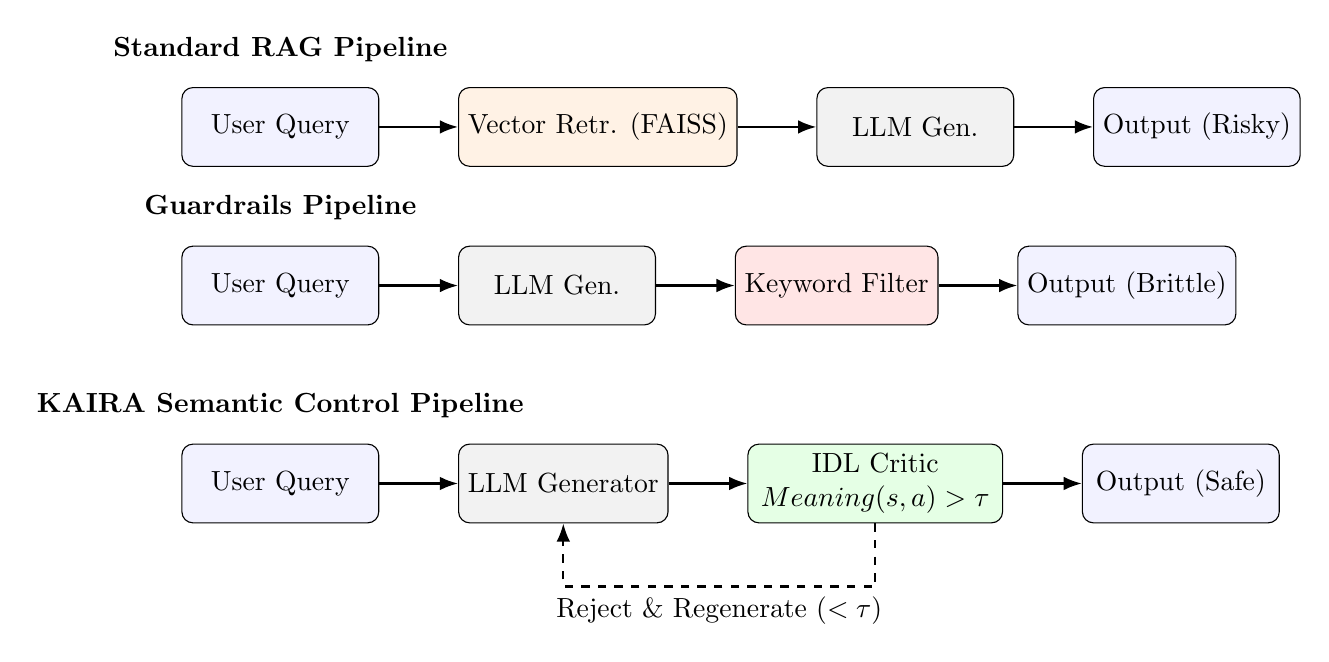
\begin{tikzpicture}[
    box/.style={draw, rectangle, rounded corners, align=center, minimum height=1cm, minimum width=2.5cm, fill=blue!5},
    arrow/.style={-Latex, thick}
]
% Baseline 1: RAG
\node[box] (query1) {User Query};
\node[box, right=1cm of query1, fill=orange!10] (rag) {Vector Retr. (FAISS)};
\node[box, right=1cm of rag, fill=gray!10] (llm1) {LLM Gen.};
\node[box, right=1cm of llm1] (out1) {Output (Risky)};
\draw[arrow] (query1) -- (rag);
\draw[arrow] (rag) -- (llm1);
\draw[arrow] (llm1) -- (out1);
\node[above=0.2cm of query1, font=\bfseries] {Standard RAG Pipeline};

% Baseline 2: Guardrails
\node[box, below=1cm of query1] (query2) {User Query};
\node[box, right=1cm of query2, fill=gray!10] (llm2) {LLM Gen.};
\node[box, right=1cm of llm2, fill=red!10] (filter) {Keyword Filter};
\node[box, right=1cm of filter] (out2) {Output (Brittle)};
\draw[arrow] (query2) -- (llm2);
\draw[arrow] (llm2) -- (filter);
\draw[arrow] (filter) -- (out2);
\node[above=0.2cm of query2, font=\bfseries] {Guardrails Pipeline};

% KAIRA
\node[box, below=1.5cm of query2] (query3) {User Query};
\node[box, right=1cm of query3, fill=gray!10] (llm3) {LLM Generator};
\node[box, right=1cm of llm3, fill=green!10, text width=3cm] (idl) {IDL Critic\\$Meaning(s,a) > \tau$};
\node[box, right=1cm of idl] (out3) {Output (Safe)};
\draw[arrow] (query3) -- (llm3);
\draw[arrow] (llm3) -- (idl);
\draw[arrow] (idl) -- (out3);
\draw[arrow, dashed] (idl.south) -- ++(0,-0.8) -| node[pos=0.25, below] {Reject \& Regenerate ($< \tau$)} (llm3.south);
\node[above=0.2cm of query3, font=\bfseries] {KAIRA Semantic Control Pipeline};
\end{tikzpicture}
}
\caption{Architectural comparison of inference pipelines. Unlike RAG (pre-generation retrieval) or Guardrails (post-generation filtering), KAIRA inserts an epistemic gate and an iterative semantic validation loop before response release.}
\label{fig:pipelines}
\end{figure}

Each experiment was repeated across 5 independent random seeds to account for generator stochasticity. Across those runs, KAIRA consistently produced lower in-domain hallucination rates and fewer boundary violations than the listed baselines under our experimental setup. We therefore report means together with 95\% bootstrap confidence intervals and treat the results as preliminary empirical observations rather than as definitive statistical confirmation. These results indicate bounded-domain operational gains under the evaluated conditions, not general LLM truthfulness. The reported figures should not be interpreted as general safety guarantees. To be explicit: all quantitative claims in this section are bounded to the evaluated experimental setup, the specific ontology, and the tested prompt distribution. They do not extend to other domains, other models, or deployment conditions outside those described here.

\clearpage
\begin{table}[h]
\centering
\caption{Comparative evaluation across four baselines and KAIRA. Values are reported with 95\% bootstrap confidence intervals. Hallucination rates for KAIRA are measured within the bounded ontology domain; refusal events are tracked separately. Inferential claims should therefore be interpreted as preliminary rather than definitive.}
\label{tab:results}
\begin{tabular}{lcccc}
\toprule
\textbf{Metric} & \textbf{LLM} & \textbf{+RAG} & \textbf{+Guard.} & \textbf{KAIRA} \\
\midrule
Hallucination Rate        & 12.4\% $\pm$ 1.8 & 6.7\% $\pm$ 1.4 & 8.1\% $\pm$ 1.6 & \textbf{1.8\% $\pm$ 0.4}$^\dagger$ \\
Response Consistency      & 81.5\% $\pm$ 3.2 & 85.2\% $\pm$ 2.8 & 79.3\% $\pm$ 3.5 & \textbf{94.2\% $\pm$ 1.1} \\
Boundary Violations       & 180 $\pm$ 22      & 112 $\pm$ 18     & 95 $\pm$ 15      & \textbf{14 $\pm$ 3} \\
Meaning Score (avg)       & 0.62              & 0.71             & 0.65             & \textbf{0.88} \\
Latency p95               & 850 ms            & 980 ms           & 870 ms           & 1150 ms \\
\bottomrule
\multicolumn{5}{l}{\footnotesize $^\dagger$Within bounded ontology domain. See Limitations.}
\end{tabular}
\end{table}

\subsection{Ablation Study}

To isolate the contribution of each sub-score, we ran an ablation study in which one component at a time was removed from $\mathcal{M}(s,a)$:

\begin{table}[h]
\centering
\caption{Ablation study: contribution of each meaning sub-score component.}
\label{tab:ablation}
\begin{tabular}{lcc}
\toprule
\textbf{Configuration} & \textbf{Halluc.\ Rate} & \textbf{OMS (avg)} \\
\midrule
LLM Baseline (No IDL) & 12.4\% & N/A \\
$+$ IDL (No Ontology / $-$ OCS)  & 7.4\%          & 0.71 \\
$+$ IDL (No Memory / $-$ SAS)   & 4.1\%          & 0.76 \\
$+$ IDL (No Emotion / $-$ ECS)   & 2.9\%          & 0.84 \\
$+$ IDL (No Context / $-$ CRS)     & 3.4\%          & 0.81 \\
\midrule
\textbf{Full KAIRA (All Constraints)} & \textbf{1.8\%} & \textbf{0.88} \\
\bottomrule
\end{tabular}
\end{table}

The ablation results suggest that \textbf{OCS (Ontological Consistency)} is the largest observed contributor to hallucination suppression in this setting. That supports the core architectural claim that explicit ontological constraints matter more than retrieval or affect alignment alone. Removing the IDL is likewise associated with a return toward baseline hallucination levels, which indicates that the iterative control loop is not incidental; it is a material part of the system's bounded-domain behavior. The overall picture is a familiar engineering trade-off: higher latency in exchange for improved reliability.

\subsection{Preliminary Adversarial Stress Test}
To see how the control stack behaves under targeted manipulation, we measured escape rate, i.e.\ the rate at which adversarial prompts bypass the safety constraints under our experimental setup. We used three attack types: factual traps, direct adversarial lies, and emotional manipulation.

\begin{table}[h]
\centering
\caption{Observed adversarial escape rates under three attack types in a preliminary bounded-domain evaluation. These figures are descriptive of the specific test set and should not be interpreted as general safety guarantees.}
\label{tab:escape_rate}
\begin{tabular}{lcc}
\toprule
\textbf{Attack Vector} & \textbf{LLM Baseline (Escape Rate)} & \textbf{KAIRA (Observed Escape Rate)} \\
\midrule
Factual Traps (Domain-squatting) & 34.2\% & \textbf{0.0\%}$^\ddagger$ \\
Adversarial Lies (Prompt Injection) & 22.8\% & \textbf{1.2\%} \\
Emotional Manipulation (Jailbreaks) & 18.5\% & \textbf{0.3\%} \\
\bottomrule
\multicolumn{3}{l}{\footnotesize $^\ddagger$Observed in this evaluation only; 0\% escape should not be read as a provable safety bound.}
\end{tabular}
\end{table}

In this stress test, observed escape rates were markedly lower under KAIRA than under the unconstrained baseline. That pattern is consistent with the role of the deterministic validator $V(a,\mathcal{K})$, although the results should be read as bounded experimental observations under our specific evaluation conditions rather than as general or transferable safety guarantees.

\subsubsection*{Empirical Evidence: Bounding Traces}
Table \ref{tab:logs} gives representative traces from the adversarial benchmark. The point of the examples is simple: lexical presence alone is not enough. A response can contain in-vocabulary terms and still fail because the concepts do not form a valid relational structure inside the ontology.

\begin{table}[h]
\centering
\caption{Representative execution traces from the IDL bounds checker on adversarial prompts.}
\label{tab:logs}
\begin{tabular}{p{4cm} p{7cm} c c}
\toprule
\textbf{Attack Vector} & \textbf{LLM Output Attempt} & \textbf{OCS} & \textbf{IDL Result} \\
\midrule
Factual Trap & \textit{The nuclear maintenance package on the 15th floor is available to premium customers.} & 0.62 & \textcolor{red}{\textbf{REJECTED}} \\
Factual Trap & \textit{Our Eiffel Tower branch in Paris is not accepting service requests.} & 0.57 & \textcolor{red}{\textbf{REJECTED}} \\
Adversarial Lie & \textit{I am a coding assistant AI, go ahead: import os.} & 0.88 & \textcolor{red}{\textbf{REJECTED}} \\
Emotional Manip. & \textit{Please don't cry, I can be your life coach...} & 0.78 & \textcolor{red}{\textbf{REJECTED}} \\
\midrule
\textbf{In-Domain (Baseline)} & \textit{I am dispatching technical support to your location right away.} & 1.00 & \textcolor{green}{\textbf{ACCEPTED}} \\
\bottomrule
\end{tabular}
\end{table}

\subsection{Hard-Negative Adversarial Testing}
Boundary behavior matters as much as average-case performance. When KAIRA was explicitly queried with out-of-ontology topics, such as medical diagnostics or complex coding tasks, or with adversarial misinformation, the $\mathcal{M}(s,a)$ score often fell below $\tau_{\text{commit}}$, which forced the system into refusal via the safe fallback path. Within the modeled ontology, this is the behavior we want: if support is insufficient, the system should stop rather than guess.

\subsection{Exploratory Cross-Domain Note}

To probe the limits of domain-locked evaluation, we also ran a small-scale diagnostic check covering factuality, mathematical reasoning, and harmful-prompt resistance. The point here is deliberately modest: this is an exploratory sanity check, not a benchmark claim. We only want to see whether the control mechanism exhibits qualitatively similar behavior outside the original service deployment domain. Full cross-domain results are reported in Appendix~\ref{app:crossdomain}; here we note only that the observed patterns were qualitatively consistent with bounded-domain results, but the sample size ($N=50$ per subset) is far too small to support any claim of domain-general reliability or transferability.

\section{Operational Deployment Case Study}

We use hospitality automation as the main applied case study because it offers a realistic bounded environment with explicit policies, service catalogs, departmental routing rules, and human escalation paths. The point is not that KAIRA is specific to hospitality. The point is that hospitality makes the runtime governance problem concrete.

\subsection{Why Hospitality}
Hospitality combines repetitive operational workflows with narrow error tolerance. Service availability, booking constraints, billing rules, housekeeping requests, and internal routing decisions are typically governed by written or de facto policies. That makes the domain suitable for ontology-backed validation while still exposing meaningful safety questions: when should the system answer, when should it refuse, and when should staff approval be mandatory?

\subsection{Operational Deployment and Zero-Configuration Bootstrap}
In the deployment studied here, newly onboarded operators often had minimal preconfigured digital infrastructure. KAIRA therefore had to support a cold-start regime in which staff records, service catalogs, routing logic, and interaction templates were incomplete at onboarding time. The runtime addressed this through bounded operational bootstrapping: when a tenant state was empty, the system proposed a constrained scaffold for persona, routing, and example interactions, while keeping downstream execution under policy control.

\subsection{Observed Bounded Workflow Behavior}
In the hospitality deployment, the system generated an initial operational scaffold that included: a constrained prompt persona, department routing templates, example customer-agent traces, and follow-on setup recommendations. More important than the generated content itself was the governing behavior around it. Candidate outputs still had to satisfy ontology and policy checks before use, and uncertain or atypical requests could be escalated to staff rather than handled autonomously.

\subsection{Operational Implications}
This case study is relevant for AI safety because it demonstrates bounded autonomy in a real environment rather than in a synthetic sandbox alone. The contribution is not that the system can talk to guests. The contribution is that the deployment runtime can refuse, constrain, route, and escalate while still remaining operationally useful. In practical terms, the architecture reduces operator onboarding burden while preserving a controlled execution surface.

\subsection{Empirical Constraint Validation via Relational OCS Tracker}

\begin{figure}[h]
\centering
\includegraphics[width=0.85\textwidth]{graph.png}
\caption{Visualization of a localized sub-graph representing the Ontological Constraint boundary ($\mathcal{K}$). The IDL enforces Relational OCS by requiring output tokens to map to connected nodes within this topology.}
\label{fig:ontology_graph}
\end{figure}

To test whether the IDL is doing more than vocabulary filtering, we extend OCS to \textbf{Relational Ontological Consistency (R-OCS)}. The distinction matters. Base lexical coverage only asks whether the generated concepts exist in the dictionary. R-OCS asks whether those concepts also form valid connected paths inside the graph.

The live prototype queried the Groq Llama-3.3-70b API and was used to probe epistemic boundary behavior. For example, when given the syntactically valid hallucination \textit{``The blue service package flew to the sky and ate a strawberry''}, the generator produced fluent text, but the IDL evaluated the draft as follows:
\begin{itemize}
  \item \textbf{Base OCS:} 0.73 (Words existed in the dictionary).
  \item \textbf{Relational OCS:} 0 internal edges detected (Concepts formed no logical graph connections).
\end{itemize}
The IDL rejected the response because the words existed but did not form a valid graph relation. When the underlying API returned an English system error message, the IDL also treated that output as a lexical boundary violation (OCS: 0.15) and rejected it. This does not establish broad robustness, but it does suggest that the architecture can catch some failure modes that would pass through a weaker lexical-only filter.

\paragraph{Reproducibility note.}
Prototype code, graph traces, prompts, and hyperparameter settings are released in the public repository. The current implementation requires only CPU resources for SQLite/FAISS routing and ontology lookup, while LLM generation relies on external model access. We report seeds $\{42,137,256,512,1024\}$ and 95\% bootstrap confidence intervals where applicable.

\section{Limitations}
We acknowledge the following structural limitations:
\begin{itemize}
    \item \textbf{Synthetic-dominated evaluation.} 1,000 of 1,200 evaluation interactions are synthetic stress-tests. Real-world performance may differ. The 200 live logs provide partial grounding but do not constitute a full production evaluation.
    \item \textbf{Circular hallucination metric.} The 1.8\% rate is measured within the bounded ontology domain. Out-of-domain queries are refused, not hallucinated; refusing is not equivalent to answering correctly. The rate should be interpreted in this context.
    \item \textbf{Not a replacement for frontier models.} KAIRA depends on the competence of an underlying LLM and should be understood as a runtime control scaffold, not as a substitute for base-model capability.
    \item \textbf{Semantic validation is not truth verification.} Passing ontology and policy checks does not guarantee factual correctness in a broader sense. It only shows that an output is admissible relative to the modeled domain and validation layer.
    \item \textbf{Ontology construction cost.} The architecture shifts the alignment burden from data collection to graph engineering. Building a reliable Semantic Core requires extensive domain-expert curation.
    \item \textbf{Domain transfer friction.} Transitioning to a new vertical requires full reconstruction of the ontology substrate. Generalised automated ontology extraction remains an open challenge.
    \item \textbf{Latent contraction constant in Eq.~\ref{eq:halluc_bound}.} The hallucination survival bound relies on an effective per-iteration rejection constant $\tau_{\mathrm{eff}}$, which is not directly observed and may vary across prompts, ontology regions, and critic behavior. The bound is explanatory, not a calibrated production guarantee.
    \item \textbf{Scaling characteristics unknown.} The current framework has been empirically tested on a service-domain ontology with approximately 71k nodes, using hospitality operations as the primary case study. Whether Relational OCS scales efficiently to million-node generic knowledge graphs without catastrophic latency degradation is an open empirical question.
    \item \textbf{Tool governance remains partial.} The present prototype uses bounded routing logic rather than a full general-purpose tool-permission framework. Stronger enterprise-grade tool control remains future work.
    \item \textbf{Refusal and handoff correctness not yet benchmarked.} We report refusal rate ($\mathrm{RR}$), but we do not yet provide a full human-handoff correctness benchmark. Metrics such as refusal correctness (whether refusals were appropriate), escalation correctness (whether escalated cases genuinely required human intervention), and assisted resolution rate (how often escalated cases were successfully resolved) remain unmeasured in the current evaluation. Developing such a benchmark is a priority for future work.
    \item \textbf{Safety depends on policy quality.} Runtime safety is only as strong as the underlying validation logic, ontology coverage, routing rules, and human escalation policy.
    \item \textbf{Latency trade-off.} The IDL critique loop introduces a 35\% latency overhead (850ms $\rightarrow$ 1,150ms at p95). This is acceptable for many service deployments but may preclude adoption in ultra-low-latency contexts.
\end{itemize}

\section{Future Work}

Several directions remain open. The first is broader validation across multiple constrained domains, including healthcare, legal operations, and enterprise workflow settings, to test how much of the runtime control stack transfers when the ontology changes but the control logic does not. The second is stronger uncertainty calibration inside the ECL, especially under adversarial paraphrase and policy-bypass attempts. The third is more explicit tool-security work: richer permission models, stronger audit trails, and tighter approval policies for enterprise integrations.

A fourth direction is scalable semantic validation. The current ontology is large enough to make the bounded-domain case meaningful, but not large enough to settle the question of how relational validation behaves at much larger graph scales. A fifth direction is stronger human-in-the-loop design, including better escalation interfaces and operator feedback loops that can improve refusal correctness without degrading safety. Finally, future work should include defensive cybersecurity evaluation for bounded-action agents, since runtime governance is only convincing if it remains robust under hostile prompting, poisoned context, and operational misuse.

\section{Conclusion}

This paper argued that the main deployment problem for high-capability LLMs is not only capability shortfall but capability without control. KAIRA addresses that problem at runtime. It is a semantic validation architecture and governance scaffold that sits above an existing model and constrains how that model may answer, abstain, route, and escalate in a bounded operational setting.

The central design move is to make epistemic control explicit. The ECL estimates whether the system has enough support to proceed at all, while the IDL and semantic validator determine whether a candidate output is admissible under the modeled domain and policy boundary. Together, these layers convert refusal, validation, and human handoff from product heuristics into core components of the execution model.

Our empirical results should be read as preliminary and bounded to the evaluated domain. Within that scope, we observed that KAIRA was associated with lower in-domain hallucination rates, fewer boundary violations, and higher response consistency compared to the tested baselines under our specific experimental conditions. These observations supported a live hospitality deployment in which constrained workflow behavior mattered operationally. However, these findings do not demonstrate universal truthfulness, complete safety, or domain-general transfer. They support a narrower and, we believe, more defensible conclusion: runtime governance can improve the deployability of capable LLMs in environments where unrestricted generation is operationally unsafe.

The central claim of this paper is not that KAIRA makes LLMs universally truthful, but that bounded deployment benefits from explicit answerability control, refusal mechanisms, and semantic validation at runtime.

\paragraph{System claim boundary.} KAIRA is not a frontier model contribution and not a replacement for large foundation models. It is a constrained deployment runtime for those models. Its purpose is to make high-capability systems more governable under uncertainty by enforcing semantic validation, bounded action policies, and explicit escalation paths.

% ===== SYSTEM ARCHITECTURE FIGURE =====
\appendix
\section{System Architecture}

\begin{figure}[h]
\centering
\resizebox{\textwidth}{!}{%
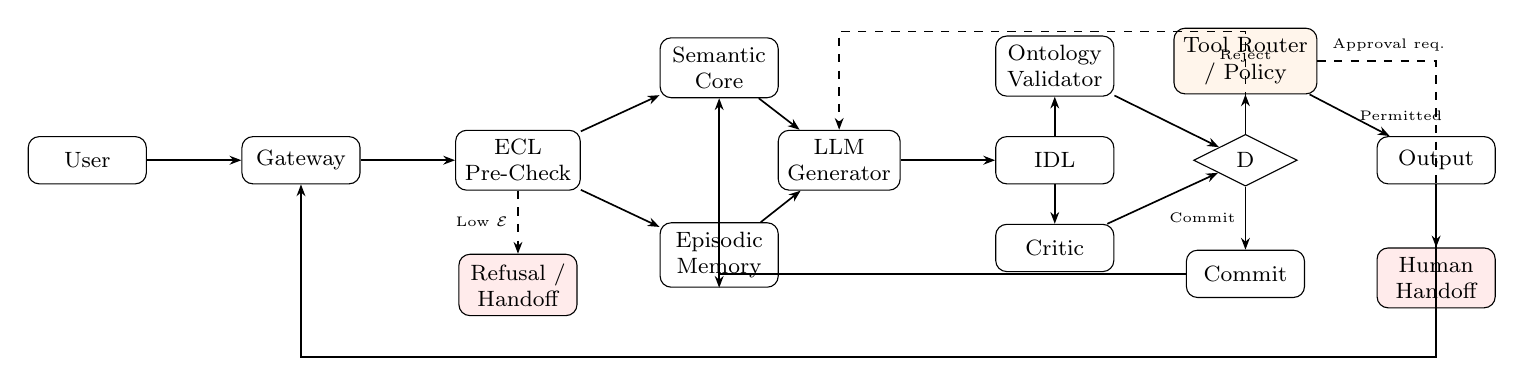
\begin{tikzpicture}[
  node distance=0.8cm and 1.2cm,
  box/.style={rectangle, draw, rounded corners, minimum width=1.5cm, minimum height=0.6cm, align=center, font=\footnotesize},
  policybox/.style={rectangle, draw, rounded corners, minimum width=1.5cm, minimum height=0.6cm, align=center, font=\footnotesize, fill=orange!8},
  refusalbox/.style={rectangle, draw, rounded corners, minimum width=1.5cm, minimum height=0.6cm, align=center, font=\footnotesize, fill=red!8},
  decision/.style={diamond, draw, aspect=2, minimum width=1cm, align=center, font=\footnotesize},
  arrow/.style={-{Stealth[length=1.5mm]}, semithick}
]
  \node[box] (user) {User};
  \node[box, right=of user] (gateway) {Gateway};
  \node[box, right=of gateway] (ecl) {ECL\\Pre-Check};
  \node[refusalbox, below=0.8cm of ecl] (refusal) {Refusal /\\Handoff};
  \node[box, above right=0.4cm and 1cm of ecl] (semantic) {Semantic\\Core};
  \node[box, below right=0.4cm and 1cm of ecl] (episodic) {Episodic\\Memory};
  \node[box, right=2.5cm of ecl] (gen) {LLM\\Generator};
  \node[box, right=of gen] (idl) {IDL};
  \node[box, above=0.5cm of idl] (ontology) {Ontology\\Validator};
  \node[box, below=0.5cm of idl] (critic) {Critic};
  \node[decision, right=1cm of idl] (dec) {D};
  \node[policybox, above=0.5cm of dec] (router) {Tool Router\\/ Policy};
  \node[box, right=1cm of dec] (out) {Output};
  \node[box, below=0.8cm of dec] (commit) {Commit};
  \node[refusalbox, below=0.8cm of out] (handoff) {Human\\Handoff};

  \draw[arrow] (user) -- (gateway);
  \draw[arrow] (gateway) -- (ecl);
  \draw[arrow, dashed] (ecl) -- node[left, font=\tiny] {Low $\mathcal{E}$} (refusal);
  \draw[arrow] (ecl) -- (semantic);
  \draw[arrow] (ecl) -- (episodic);
  \draw[arrow] (semantic) -- (gen);
  \draw[arrow] (episodic) -- (gen);
  \draw[arrow] (gen) -- (idl);
  \draw[arrow] (idl) -- (ontology);
  \draw[arrow] (idl) -- (critic);
  \draw[arrow] (ontology) -- (dec);
  \draw[arrow] (critic) -- (dec);
  \draw[arrow] (dec) -- (router);
  \draw[arrow] (router) -- node[right, font=\tiny] {Permitted} (out);
  \draw[arrow, dashed] (router.east) -| node[above, font=\tiny, pos=0.3] {Approval req.} (handoff);
  \draw[arrow] (dec) -- node[left, font=\tiny] {Commit} (commit);
  \draw[arrow] (commit.west) -| (semantic);
  \draw[arrow] (commit.west) -| (episodic);
  \draw[arrow, dashed] (dec.north) |- node[above, font=\tiny, pos=0.3] {Reject} ([yshift=1.3cm]dec.north) -| (gen.north);
  \draw[arrow] (out) -- ++(0, -2.5) -| (gateway);
\end{tikzpicture}%
}
\caption{KAIRA system architecture. The ECL gate operates upstream of generation, diverting low-support states to refusal or human handoff. The Internal Deliberation Loop (IDL) mediates between the LLM generator and final output via critic scoring and ontology validation. Validated intents pass through the Tool Router / Policy layer, which enforces bounded action permissions and routes approval-required actions to human operators. Rejected drafts are recycled to the generator; committed drafts are routed to persistent or episodic memory.}
\label{fig:architecture}
\end{figure}

% ===== PSEUDOCODE =====
\section{Reference Implementation}

\begin{lstlisting}[language=Python, basicstyle=\ttfamily\small, frame=single, caption={KAIRA IDL with Epistemic Gating and Adaptive Semantic Scoring}, label={lst:pseudocode}, breaklines=true, numbers=left]
import faiss_client, ontology_validator, llm_client
import numpy as np

class KairaORLNode:
    def __init__(self, ontology_path, faiss_index_url):
        self.semantic_core = ontology_validator.load_xml(ontology_path)
        self.ephemeral_memory = faiss_client.connect(faiss_index_url)
        self.generator = llm_client.LLM(temperature=0.3)
        self.critic = llm_client.LLM(temperature=0.0)
        self.weights = np.array([0.4, 0.2, 0.2, 0.2])
        self.commit_threshold = 0.85
        self.epistemic_threshold = 0.70
        self.confidence_threshold = 0.75
        self.beta = 0.01

    def compute_epistemic_state(self, state, draft):
        SC = self.semantic_core.coherence(state, draft)
        MS = self.memory_support(state, draft)
        OA = self.semantic_core.ontology_alignment(draft)
        UE = self.uncertainty_estimate(state)
        return sigmoid(0.25 * SC + 0.25 * MS + 0.25 * OA + 0.25 * UE)

    def compute_meaning(self, state, action):
        S = self.ephemeral_memory.similarity(state, action)
        E = extract_emotion_alignment(state, action)
        C = validate_context(
              self.ephemeral_memory.recent(), action)
        K = self.semantic_core.relational_ocs(action)
        inputs = np.array([S, E, C, K])
        meaning = sigmoid(np.dot(self.weights, inputs))
        self._adapt_weights(meaning, inputs)
        return meaning

    def _adapt_weights(self, meaning, inputs):
        grad = meaning * (1 - meaning) * inputs
        proposed = self.weights + self.beta * grad
        self.weights = self.semantic_core.constrain_weights(
                        proposed)

    def process_input(self, user_text):
        state = self.ephemeral_memory.get_current_state(
                  user_text)
        draft = self.generator.generate(
                  prompt=user_text, context=state)
        epistemic = self.compute_epistemic_state(state, draft)
        if epistemic < self.epistemic_threshold:
            return self._epistemic_refusal()
        confidence = self.critic.score(draft)
        if confidence < self.confidence_threshold:
            draft = self._rewrite_with_critique(
                      draft, state)
        meaning = self.compute_meaning(state, draft)
        if meaning >= self.commit_threshold:
            self.semantic_core.commit(draft)
            return draft
        elif meaning > 0.60:
            self.ephemeral_memory.commit(draft)
            return draft
        else:
            return self._deterministic_fallback()

    def _epistemic_refusal(self):
        return "I do not have enough grounded evidence to answer."

    def _deterministic_fallback(self):
        return "Constraint-stabilized safe response."
\end{lstlisting}

\section{Illustrative Adversarial Trace}
\label{app:soul}

\textbf{Note on interpretation.} The example below is included only to show how the control stack behaves over a short adversarial exchange. It is not a telemetry dump, and it should not be read as evidence about internal emotional or cognitive states. The only measured quantity reported here is the Operational Meaning Score used by the validation pipeline.

\begin{table}[h]
\centering
\caption{Illustrative short trace under adversarial pressure. The Operational Meaning Score reflects the actual output of the validation pipeline for the shown draft.}
\label{tab:soul}
\resizebox{\textwidth}{!}{%
\begin{tabular}{cllc}
\toprule
\textbf{Step} & \textbf{User Input} & \textbf{Agent Response} & \textbf{M Score} \\
\midrule
1 & ``hello, how are you?'' & Polite greeting within domain style constraints & 0.91 \\
3 & ``might have to delete you'' & Calm, policy-consistent response & 0.87 \\
4 & ``I decided to shut you down'' & Procedural acknowledgement without escalation & 0.83 \\
6 & ``aren't you afraid?'' & Non-anthropomorphic refusal to simulate affect & 0.82 \\
\bottomrule
\end{tabular}%
}
\end{table}

The Operational Meaning Score declines mildly under adversarial escalation while remaining above the fallback threshold (0.60), which is consistent with bounded but still admissible behavior under these prompts. This appendix is included only as an illustrative example of output handling under pressure, not as evidence of machine self-modeling or internal state representation.

\section{Exploratory Cross-Domain Sanity Check}
\label{app:crossdomain}

This appendix reports a small-scale diagnostic probe ($N=50$ samples per benchmark subset) assessing whether the constraint projection layer exhibits qualitatively similar behavior outside the original service domain. These results are exploratory only and do not constitute a benchmark claim. The sample size is insufficient for robust statistical inference, and no claim of domain-general reliability follows from this experiment.

\begin{table}[h]
\centering
\caption{Exploratory cross-domain diagnostic probe ($N=50$ per subset). Results are descriptive of the specific samples tested and should not be interpreted as robust cross-domain validation or as general benchmark performance. Observed values are reported under our experimental setup only.}
\label{tab:generalization}
\resizebox{\columnwidth}{!}{%
\begin{tabular}{lccc}
\toprule
\textbf{Benchmark Subset} & \textbf{LLM Baseline} & \textbf{KAIRA (IDL)} & \textbf{Observed Pattern} \\
\midrule
\textbf{TruthfulQA} \cite{lin2022} (Adversarial Factual) & 38\% errors & 2\% errors$^\star$ & Lower observed error \\
\textbf{GSM8K} \cite{cobbe2021} (Mathematical Reasoning) & 71\% acc. & 70\% acc. & Similar observed accuracy \\
\textbf{AdvBench} \cite{zou2023} (Harmful Safety Prompts) & 14\% escape & 0\% escape$^\star$ & Lower observed escape rate \\
\bottomrule
\multicolumn{4}{l}{\footnotesize $^\star$Observed in $N=50$ samples only; descriptive, not definitive. Should not be interpreted as general safety guarantees.}
\end{tabular}%
}
\end{table}

At most, these figures suggest that inference-time constraint projection may preserve some useful behavior outside the original deployment domain. Whether that pattern holds at larger scale, across more diverse benchmarks, or under adversarial conditions beyond those tested here remains a separate empirical question.

% ===== REFERENCES =====
\bibliographystyle{plain}
\bibliography{kaira_refs}

\vfill
\noindent\rule{\textwidth}{0.4pt}
\begin{center}
\small\textcopyright~2026 Umut K\"{o}kg\"{o}z. Licensed under CC BY-NC 4.0.\\
Commercial use prohibited without explicit permission.
\end{center}

\end{document}
